\chapter{Implementation of Highest Delivery Guarantee} \label{chap:implementation}
As elaborated in section \ref{section:semantics}, Apache Kafka and Apache Pulsar can support exactly-once semantics as the highest guarantee while on NATS Streaming, only at-least-once delivery semantics can be achieved. In order to analyze in more detail how the platforms achieve their highest level of delivery guarantee, especially exactly-once semantics, a small use case is implemented on all three platforms. Apart from providing insights into the internal workflow of the platforms, this can also serve as a reference for realizing the delivery guarantee on the platforms in production. 
\section{Overview}
For the realization of delivery guarantee, a simple use case of banking transactions is used. Transactional activities of customers are recorded as events and published to the ESP platform. These raw events are transformed and the values of all transactions are aggregated to generate the current account balance for each user. The overview of event flow and the main components in the implementation is showed in figure \ref{fig:impusecase}.

To simulate the incoming events from customers, an event generator is implemented. The generator reads events from a CSV file which is prepared in advanced with data of 1000 transactional events. The generator then publishes these events to an event stream named \emph{raw-event}. Moreover, the event generator also checkpoints the line number in the CSV file of the published event to another stream named \emph{reading-position} on the ESP platform. In this way, when the event generator restarts, it can retrieve this checkpoint and resume the reading on the source file at the right position. 

To transform raw event, a stream processor is implemented. This component will ingest data from \emph{raw-event} stream, extract and transform the transactional value based on the event type and publish this transformed event back into another stream \emph{transformed-event}. This component will rely on the built-in mechanism of the ESP platform to manage the reading position on the \emph{raw-event} stream.



\begin{figure}
\begin{adjustwidth}{-1cm}{}
	\centering
	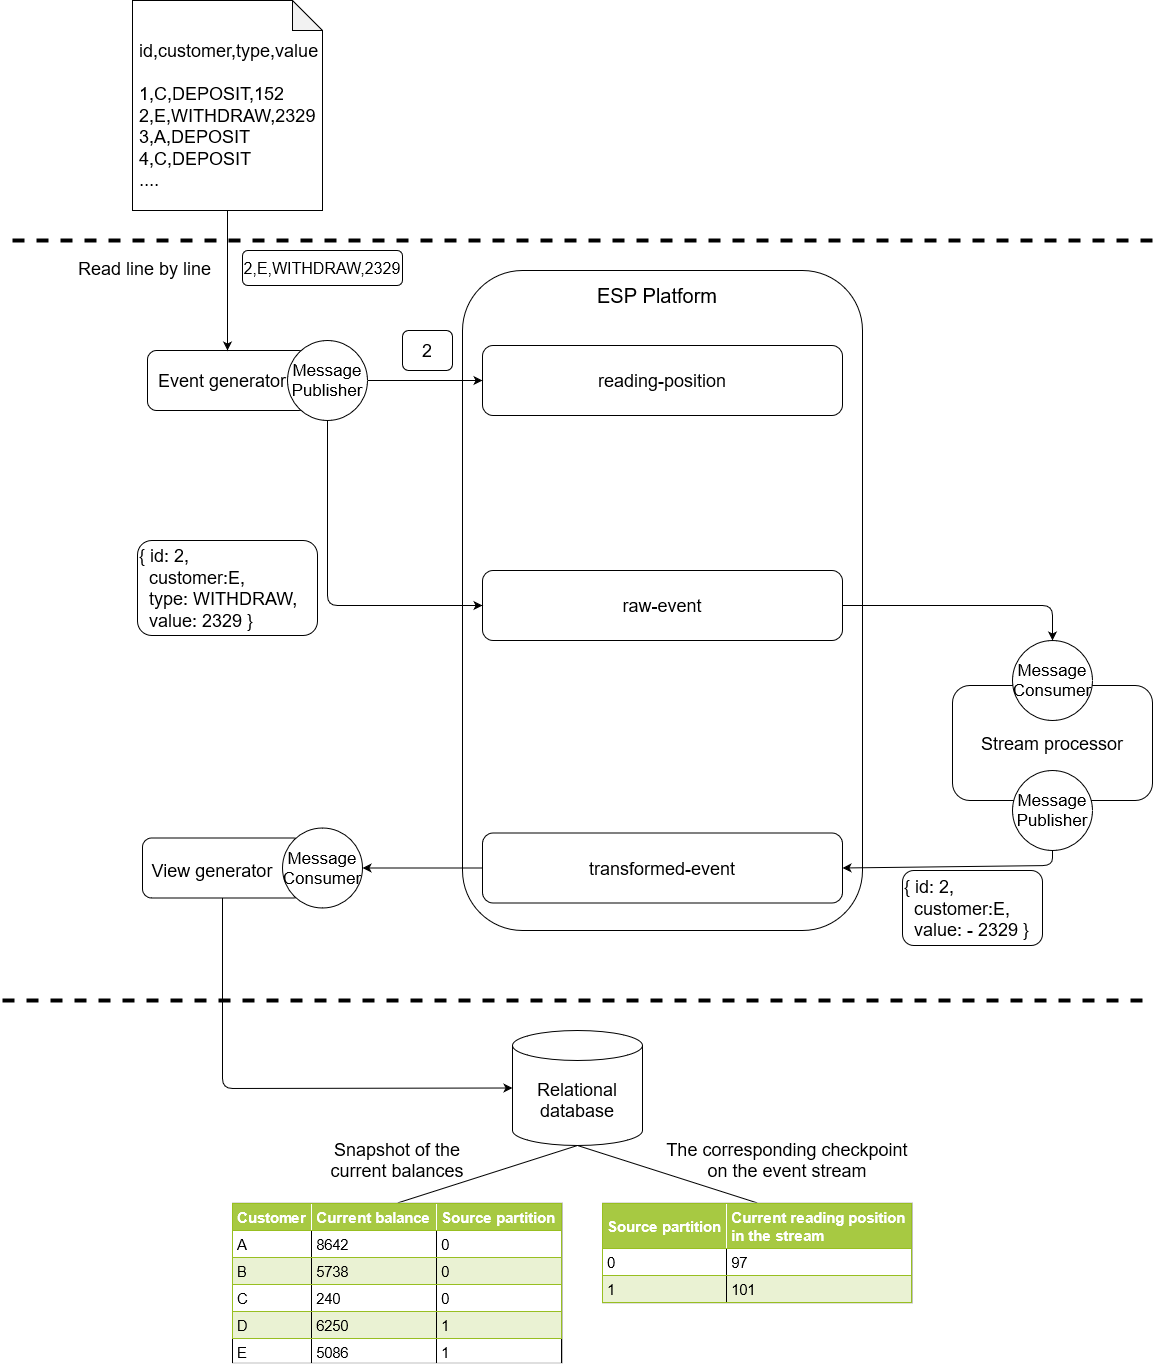
\includegraphics[width=18cm,height=\textheight]{images/implementation-use-case-1.png}
	\caption{Use case to implement delivery guarantee on the platforms.}
	\label{fig:impusecase}
\end{adjustwidth}
\end{figure}


Finally at the end of the event streams pipeline, the view generator component will accumulate the transactional values of each user and persist the resulted current balance to a PostgreSQL relational database. In addition, the view generator also commit the corresponding reading position on the source stream \emph{transformed-event} to the database so that it can fetch this value and resume the consumption on the stream accordingly upon restarting.


With this setup, message duplication can be easily detected because any transactional event which is processed more than once by any of the three processing components will result in different final current balances. To verify that the configuration and implementation is correct on each platform to achieve the highest message delivery guarantee, different failure scenarios are setup. The final current balances in these scenarios will be verified against the result from the reference scenario without failure.

 
\subsection{Failure scenarios}  \label{subsection:failurescenarios}
To focus on the components which interact directly with the platform, the source CSV file with events data and the relational database is assumed to be reliable with no failure. Moreover, the platforms are configured to be fault-tolerant with redundancies and assumed to be resilient to failures.  Failure scenarios will only be derived for three components: event generator, stream processor, and view generator.

\begin{figure}[h]
	\centering
	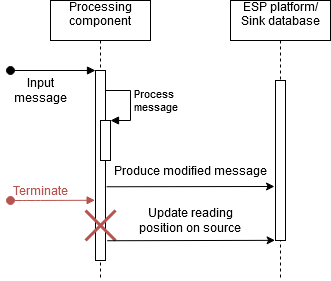
\includegraphics[width=7cm,height=7cm]{images/reading-position-fail.png}
	\caption{Failure scenarios \emph{event-generator-crash}, \emph{stream-processor-crash} and \emph{stream-aggregator-crash}.}
	\label{fig:scenarioreadingposition}
\end{figure}

These components all have the processing cycle of an event as read-modify-write. After writing the modified event, these components must successfully update the reading position on the source system. Otherwise, failure when updating reading position can lead to the case where the last processed message will be redelivered and reprocessed when the application restarts. Three failure scenarios, namely, \emph{event-generator-crash}, \emph{stream-processor-crash} and \emph{stream-aggregator-crash}, are derived for three processing components. In each failure scenario, one processing component along the processing pipeline is deliberately terminated before it can checkpoint the reading position on the data source to simulate the application crash (figure \ref{fig:scenarioreadingposition}). After that, the processing component will be restarted to continue with its incomplete task.



Kafka and Pulsar support using the consumer group pattern to read a partitioned topic with multiple concurrent consumer instances (section \ref{section:patterns}). In this case, users have the option to rely on the failover mechanism of the consumer group to automatically manage and assign partitions of the topic to consumer instances in the same group. However, this can lead to the case same messages are sent and buffered on two different consumer instances when the platform transfer ownership of a partition from one consumer to another. Therefore, for Apache Kafka and Apache Pulsar, another failure scenario called \emph{duplicated-consumer} is setup.

On Kafka, whenever a consumer send a pulling request for new messages from Kafka, it will be notified about partition reassignment event if there is any. In normal condition, when the partitions are redistributed among the consumers (e.g. when a new consumer joins the consumer group), before the new consumer is notified about its newly assigned partition, the previous owner of the partition always has the chance to gracefully give up the ownership on the partition by committing the offset number of processed messages \cite{kafkaconsumerimplement}. Kafka handles the coordination of this transition process transparently to users. Therefore, same messages will not be delivered to two different consumers in this case. 

However, ownership on a partition can be revoked before the owning consumer is notified. This is the case when the consumer is stalled for some reason (e.g. garbage collection pause, some messages take longer to process than expected) and fails to send new messages pulling request within the permitted interval. In this case, the consumer will be removed from the group by Kafka and its partition will be reassigned to another consumer in the group. As a result, the messages whose offset numbers have not been committed by old consumer will be redelivered to the new one leading to message duplication on two instances. This scenario can be simulated by simply pausing a consumer instance in the consumer group after it has pulled a new batch of messages and before it starts to process and commit offset for these messages until Kafka deems this consumer to be disconnected (figure \ref{fig:kafkascenario}). 

\begin{figure}[t!]
	\begin{adjustwidth}{-2cm}{-2cm}
	\centering

	\begin{subfigure}[t]{0.49\linewidth}
		\centering
		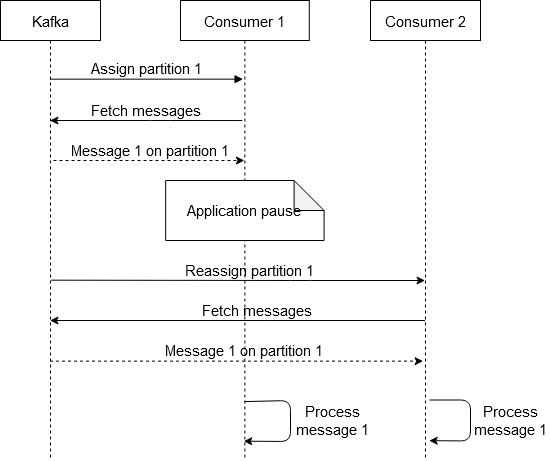
\includegraphics[width=\linewidth]{images/kafka-duplicated-scenario.png}
		\caption{Failure scenario \emph{duplicated-consumer} on Kafka when a partition is reassigned without notifying the previous owning consumer.}
		\label{fig:kafkascenario}
	\end{subfigure}
	\begin{subfigure}[t]{0.49\linewidth}
		\centering
		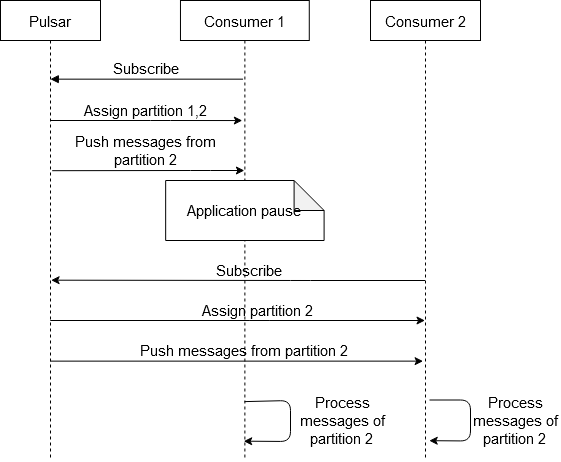
\includegraphics[width=\linewidth]{images/pulsar-duplicated-scenario.png}
		\caption{Failure scenario \emph{duplicated-consumer} on Pulsar when a new consumer joins the failover subscription.}
		\label{fig:pulsarscenario}
	\end{subfigure}
\end{adjustwidth}
	\caption{Failure scenario \emph{duplicated-consumer} on Kafka and Pulsar.}
	\label{fig:failurescenario}
\end{figure}

The failure scenario \emph{duplicated-consumer} can also occur with Pulsar. When a consumer subscribe to a Pulsar topic, messages on all topic assigned to this consumer will be pushed to a local queue until it is full \cite{pulsarbinaryprotocol}. When the consumer has consumed and acknowledged half of the buffered messages, new messages will be delivered. When a new consumer joins the same failover subscription, Pulsar broker will assign some topic partitions to it for load balancing. In this case, if the old consumer has not processed and acknowledged all messages of the reassigned partition on its queue, these messages will be redelivered again to the new consumer which causes message duplication on the queue of two consumers. This scenario can be provoked by introduced a small delay into the first consumer instance before it can start to process the messages on its local queue to give the second consumer instance enough time to join the subscription and receive the unprocessed messages again. This is illustrated in figure \ref{fig:pulsarscenario}.

The \emph{duplicated-consumer} scenario will be realized on the stream processor component where the consuming and producing of messages are done within the protection scope of the platform. For the view generator component which reads input from the ESP platform and writes output data to an external data sink, in order to have exactly-once semantics with this scenario, the gap between the platform and the data sink varies and must be bridged differently with different types of external system.

\begin{table}[]
	\begin{adjustwidth}{-1cm}{}
	\centering
	\begin{tabular}{|l|l|l|l|}
		\hline
		& Event generator                                                          & Stream processor                                                                                                                        & View generator                                                           \\ \hline
		\textit{event-generator-crash}  & \begin{tabular}[t]{@{}l@{}}one instance\\ crash and restart\end{tabular} & \begin{tabular}[t]{@{}l@{}}one instance \\ no failure\end{tabular}                                                                      & \begin{tabular}[t]{@{}l@{}}one instance\\ no failure\end{tabular}        \\ \hline
		\textit{stream-processor-crash} & \begin{tabular}[t]{@{}l@{}}one instance\\ no failure\end{tabular}        & \begin{tabular}[t]{@{}l@{}}one instance\\ crash and restart\end{tabular}                                                                & \begin{tabular}[t]{@{}l@{}}one instance\\ no failure\end{tabular}        \\ \hline
		\textit{view-generator-crash}   & \begin{tabular}[t]{@{}l@{}}one instance\\ no failure\end{tabular}        & \begin{tabular}[t]{@{}l@{}}one instance\\ no failure\end{tabular}                                                                       & \begin{tabular}[t]{@{}l@{}}one instance\\ crash and restart\end{tabular} \\ \hline
		\textit{\begin{tabular}[t]{@{}l@{}}duplicated-consumer\\ (Kafka and Pulsar only)\end{tabular}}   & \begin{tabular}[t]{@{}l@{}}one instance\\ no failure\end{tabular}        & \begin{tabular}[t]{@{}l@{}}two instances \\ first instance: is delayed\\ second instance: no failure \end{tabular} & \begin{tabular}[t]{@{}l@{}}one instance\\ no failure\end{tabular}        \\ \hline
	\end{tabular}
	\label{fig:failurescenariostable}
	\end{adjustwidth}
	\caption{Summary of 4 failure scenarios.}
\end{table}

\section{Implementation}
\subsection{Clients}
The three main components are implemented with the low level Java client APIs of the platforms. Consumer clients of the platforms are used to subscribe and read messages on the streams while producer clients are used to publish messages to the platforms.

\textbf{Event generator and Stream processor}

\begin{figure}[ht!]
	\begin{adjustwidth}{-1cm}{-1cm}
	\centering
	\begin{minipage}[t]{.48\linewidth}
		\centering
		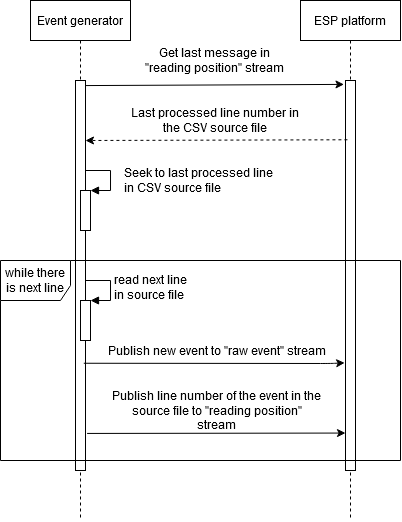
\includegraphics[width=\linewidth]{images/implement-event-generator.png}
		\caption{Sequence diagram of event generator component.}
		\label{fig:implementeventgenerator}
	\end{minipage}%
	\hfill
	\begin{minipage}[t]{.48\linewidth}
		\centering
		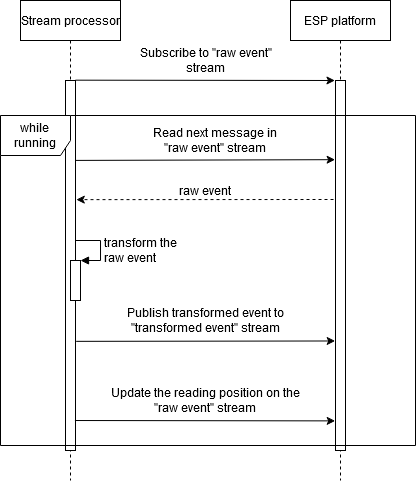
\includegraphics[width=\linewidth]{images/implement-stream-processor.png}
		\caption{Sequence diagram of stream processor component.}
		\label{fig:implementstreamprocessor}
	\end{minipage}
	\end{adjustwidth}
\end{figure}

Figures \ref{fig:implementeventgenerator} and \ref{fig:implementstreamprocessor} show the sequence diagrams of the event generator and the stream processor respectively. With Apache Kafka and Apache Pulsar, to achieve exactly-once semantics with these two components,  the two operations to publish events and update the reading position on the data source must be atomically combined with the transaction features of the two platforms. 

Listing \ref{lst:kafkastreamprocessor} shows part of the source code of the stream processor component for Kafka. The transaction, in which transformed events are published to \emph{transformed-event} topic and the offset numbers of consumed messages on \emph{raw-event} topic are committed to Kafka, is started on line 13 and committed on line 27. 

\lstinputlisting[label={lst:kafkastreamprocessor},language=Java,caption={Kafka stream processor with the transaction feature.}]{chapters/implementation/KafkaStreamProcessor.java} 

To ensure exactly-once semantics, Kafka has fencing mechanism in its transactions to prevent duplication of messages and notify users by throwing back exceptions. When there is two producer instances with the same ID trying to publish messages to Kafka, requests from older instance will be rejected by Kafka and a \emph{ProducerFencedException} will be returned to this instance. When a temporarily disconnected application is replaced by a newer instance and the old instance later reconnects, this could lead to two instances sending message simultaneously. This fencing mechanism helps prevent that scenario. 

Fencing mechanism of Kafka also prevents messages duplication when partition reassignment occurs within a consumer group \cite{kafkatransctionscaleproducer}. When the offset number of source topic is committed in a transaction (as in line 23 in listing \ref{lst:kafkastreamprocessor}), the metadata of the consumer which is used to read the input message must also be sent to Kafka. When this offset committing request is accepted by Kafka, the partition to which the message belongs is locked by the consumer instance declared in the request. If partition reassignment is triggered after the lock is obtained, the new owner of the reassigned partition must wait until the ongoing transaction on the locked partition is either completed, aborted or timeout before it can pull new messages from Kafka. Moreover, Kafka ensures that a partition can only be locked by a consumer with up-to-date metadata. When a consumer is unaware of the latest partition reassignment, its metadata becomes obsolete and any offset committing requests with this consumer will be rejected by Kafka and a \emph{CommitFailedException} will be returned. Any stream processor instance with the consumer which is deemed disconnected by Kafka cannot publish any new message until its consumer rejoins the group and retrieves the latest metadata.

The implementation of the event generator with Kafka transaction is fairly similar. However, since the event generator reads input data from the CSV file rather than a Kafka topic, it only publishes reading position as a normal message to Kafka in the same transaction instead of committing offset number as in the stream processor.

For Apache Pulsar, listing \ref{lst:pulsarstreamprocessor} shows part of the source code for the stream processor with the transaction feature. 

\lstinputlisting[label={lst:pulsarstreamprocessor},language=Java,caption={Pulsar stream processor with the transaction feature.}]{chapters/implementation/PulsarStreamProcessor.java} 

In the transaction from line 17 to line 31, the transformed event and the acknowledgement of the corresponding raw event are sent to Pulsar as an atomic operation. Pulsar handles the case of partition reassignment within a consumer group quite differently from Kafka to ensure exactly-once semantics. When a consumer acknowledge the consumption of a message in a transaction, Pulsar locks this message for that specific consumer \cite{pulsartransaction} until the transaction is completed or aborted. If a message on a partition is locked before partition reassignment occurs, it will not be redelivered to the new owner of the partition. On the other hand, if rebalancing happens before an application instance acknowledges and obtains lock on a message, this message will be redelivered to the new owner of the partition and therefore simultaneously exists on the buffers of two different consumer instances. In this case, the first application instance to finish processing and acknowledge will obtain the lock and cause the other instance to back off with a \emph{TransactionConflictException} when it tries to acknowledge the same message. As a result, exactly-once semantics can still be guaranteed.

The transaction in Pulsar event generator is implemented similarly. Instead of acknowledging message on the source topic, the event generator update the reading position by publishing the line number of published event in the CSV file in the same transaction. 

With NATS Streaming, atomically publishing and acknowledging the consumption of multiple messages is not supported. Therefore, the event generator and stream processor are implemented according to the sequence diagrams in figures \ref{fig:implementeventgenerator} and \ref{fig:implementstreamprocessor} without any special remark.

\textbf{View generator}

Regarding the view generator component, the implementations on all three platforms are fairly similar. To interact with the relational database and map Java object to relational table, the OpenJPA which is an implementation of Java Persistence API (JPA) \cite{jpa} is used. Two entities, namely, \emph{CurrentBalance} and \emph{CurrentReadingPosition} (listings \ref{lst:currentbalance} and \ref{lst:currentreadingposition}), representing the snapshot of current balances and reading position on the source stream respectively are defined and mapped to two corresponding tables on the PostgreSQL database.   

\lstinputlisting[label={lst:currentbalance},language=Java,caption={Current balance entity.}]{chapters/implementation/CurrentBalance.java} 

In the current balance entity, apart from the customer ID and the current balance of the corresponding customer, there is an additional field which indicates the source partition to which events from this customer is published. This field is applicable in case of Kafka and Pulsar where multiple view generator instances can consume the \emph{transformed-event} topic concurrently. When an application instance is assigned a partition, it must use this source partition field to retrieve the latest snapshots of current balances of all customers on this partition. In case of NATS Streaming, topic cannot be partitioned and therefore this field will simply be assigned a default value. 


\lstinputlisting[label={lst:currentreadingposition},language=Java,caption={Current reading position entity.}]{chapters/implementation/CurrentReadingPosition.java} 
For the current reading position entity, each partition on the source topic will be mapped to a row in the database table and is uniquely identified by the partition number. In case of NATS Streaming, there is only one row with the default partition number. 


Figure \ref{fig:implementviewgenerator} illustrates the overall workflow of the view generator component.

\begin{figure}[h]
	\centering
	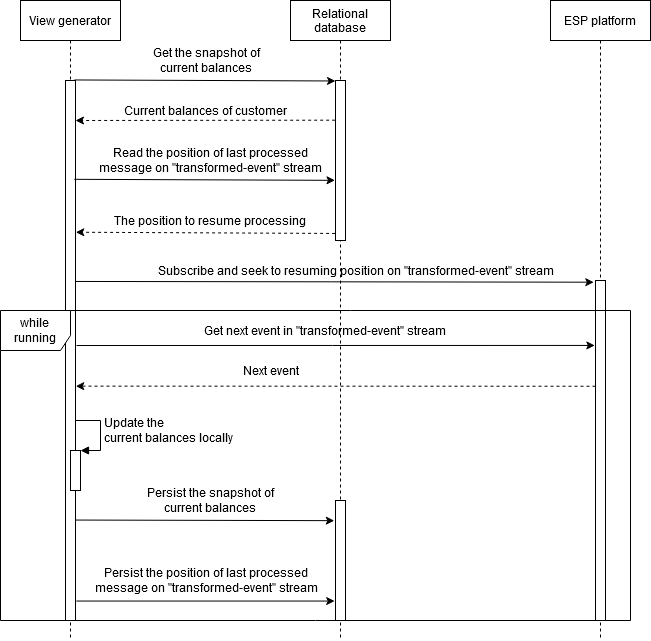
\includegraphics[width=\linewidth,height=12.6cm]{images/implement-view-generator.png}
	\caption{Sequence diagram of view generator component.}
	\label{fig:implementviewgenerator}
\end{figure}

The two operations to persist snapshot of current balances and corresponding reading position are conducted in a transaction to ensure the atomicity and guarantee exactly-once semantics in case the view generator crashes in the middle on a transaction.

\subsection{Failure injection}
To provoke failure scenarios on the processing components, custom codes are injected into the the application at runtime using Byteman tracing tool for Java \cite{byteman}. With this tool, Byteman rule can be defined to inject arbitrary code into a running application when a condition is met. 

\lstinputlisting[label={lst:bytemanrule},language=Java,caption={Example of the Byteman rule for event-generator-crash scenario on Kafka.}]{chapters/implementation/byteman.btm} 

In the example in listing \ref{lst:bytemanrule}, a Byteman rule is define to inject failure during runtime into the event generator component of Kafka. The location to which custom code is injected is defined from line 2 to 4. More specifically, when the method \emph{bytemanHook} in the class \emph{KafkaEventsGenerator} is executed, the condition defined on line 6 is checked. In this case, the 

\subsection{Running environment}
To run the failure scenarios with each platform, Docker compose is used to containerize all components and run them locally in a Docker environment. 
\section{Results and Discussion}
After running the failure scenarios, the final current balances of customers on the relational database are compared with the result from the reference scenario without failure to check for mismatched values. The results are summarized in table \ref{fig:failurescenariosresult}.
\begin{table}[h]
	\centering
	\begin{tabular}{|l|l|l|l|}
		\hline
		& Apache Kafka & Apache Pulsar & NATS Streaming \\ \hline
		\textit{event-generator-crash}  & Exactly-once & Exactly-once  & At-least-once  \\ \hline
		\textit{stream-processor-crash} & Exactly-once & Exactly-once  & At-least-once  \\ \hline
		\textit{view-generator-crash}   & Exactly-once & Exactly-once  & Exactly-once   \\ \hline
		\textit{duplicated-consumer}    & Exactly-once & Exactly-once  & Not applicable \\ \hline
	\end{tabular}
	\caption{Achieved delivery guarantees on the platforms in 4 failure scenarios.}
	\label{fig:failurescenariosresult}
\end{table}

As expected, the transactional features of Kafka and Pulsar help ensure exactly-once semantics in the case of \emph{event-generator-crash} and \emph{stream-processor-crash} failure scenarios. On the other hand, NATS Streaming can only provide at-least-once guarantee in these scenarios.  

With the \emph{view-generator-crash} scenario, exactly-once semantics is guaranteed with all three platforms. Nevertheless, this is only resulted from the support of transaction on the sink relational database and requires manual implementation on the application level to bridge the gap between the two data systems. 

Regarding the \emph{duplicated-consumer} failure scenario, the locking mechanisms of the transactions on Kafka and Pulsar are effective to guarantee exactly-once semantics even when a message is delivered and processed by two different stream processor instances when partition reassignment occurs. 

However, the transaction feature on Pulsar can potentially lead to out-of-order processing of messages on the same partition. With the Pulsar transaction, when a message in locked by a consumer instance by being acknowledged in a transaction, this message cannot be redelivered to another consumer instance or cannot be acknowledged by other consumers if it is already delivered to their local queues. However, subsequent messages on the same partition can still be processed and acknowledged by other consumers. In the scenario depicted in figure \ref{fig:pulsaroutofordertransaction}, when partition is reassigned to consumer 2 when it joins the subscription, message m1 is already locked by consumer 1 and therefore will not be pushed to consumer 2. However, when consumer 1 fails to complete the transaction, message m1 will return to unacknowledged state and will be redelivered and processed again. This causes message m1 to be processed out-of-order after message m2 and m3 even though they are on the same partition where order is guaranteed.

Moreover, this mechanism of Pulsar to let consumers race to lock messages when they have the same messages buffered locally can lead to unexpected behaviors during runtime when a partition is not guaranteed to be consumed by only one application instance at any time. Nevertheless, since this transaction feature of Pulsar is still actively developed and refined in the technical review phase, this problem could be soon resolved in future releases. 

\newpage
\begin{figure}[h]
	\centering
	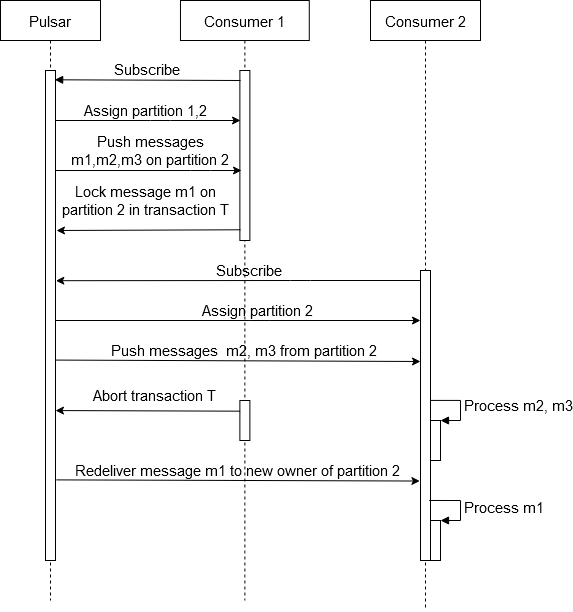
\includegraphics[width=12cm]{images/pulsar-transaction-out-of-order.png}
	\caption{Pulsar transaction can result in out-of-order processing of messages when transaction is aborted.}
	\label{fig:pulsaroutofordertransaction}
\end{figure}

The problem of out-of-order processing is well prevented on Kafka. When a consumer in the consumer group commits the offset number of a message in a transaction, the entire partition to which the message belongs is locked and any other consumer in the same group cannot fetch new messages from this partition even when it is assigned as the new owner of the partition. Only when the ongoing transaction is either completed or aborted, new owner of the partition can start to pull new messages (depicted in figure \ref{fig:kafkatransactionabort}). On the old owner of the partition, after the ongoing transaction is finished, if there is any buffered message left from the last pull request, this application instance cannot continue to commit offset numbers for them because it now has the outdated metadata of the consumer group before the partitions reassignment. When this instance sends a new pulling requests to Kafka, it receives the latest metadata as well as only messages on the partition which it is currently assigned.

\begin{figure}[h!]
	\centering
	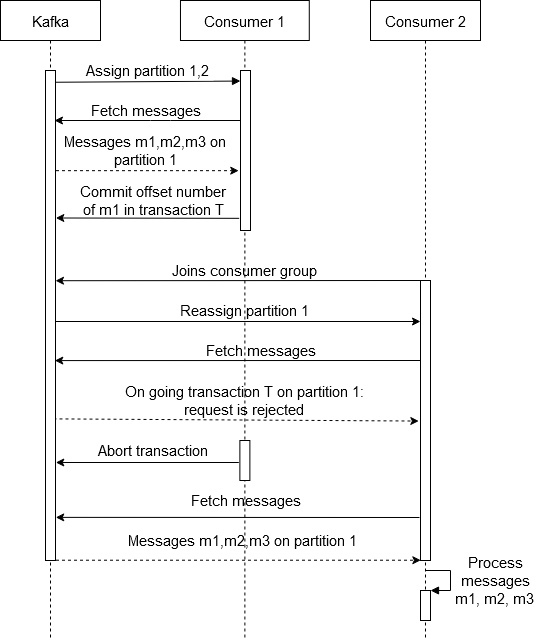
\includegraphics[width=12cm]{images/kafka-transaction-abort.png}
	\caption{Kafka transaction can prevent out-of-order processing of messages when transaction is aborted.}
	\label{fig:kafkatransactionabort}
\end{figure}

Therefore, at any time, only one consumer in a Kafka consumer group can process and commit offset numbers of messages on a partition. This mechanism of Kafka compromises the latency and availability to ensure the consistency when partition reassignment occurs. Moreover, all low-level implementation of transactions with Kafka producers and consumers as in this thesis is provided out-of-the-box with the Kafka Streams library. Users can utilize this library to focus only on the processing logic while still being able to achieve exactly-once semantics on Kafka with minimum configuration.



